
\chapter{The cell-free microbiome}

\section{Importance of the microbiome}

In an adult human, the bacteria within the colon outnumber host cell numbers by up to two orders of magnitude. This results in a frequency of bacterial genes at least 100 times greater compared with those within the human genome \cite{Brenchley:2012bm}. The importance of the microbiome is evident in studies of germ-free animals: they are more susceptible to infections and have reduced vascularity, digestive enzyme activity, muscle wall thickness. The microbiota also leads to enhanced integrity of the structural barrier of the GI tract by metabolizing dietary carbohydrates into short-chain fatty acids, metabolizes toxic and potentially carcinogenic compounds such as pyrolysates, and produces biotin, folate, and vitamin K from dietary precursors, which are then absorbed by the GI tract and circulated. In turn, numerous studies have implicated an altered balance in the composition of the microbiota (dysbiosis) in many diseases, such as obesity, celiac disease, type 2 diabetes, atopic eczema, asthma, inflammatory bowel disease (IBD), and chronic diarrhea  \cite{Brenchley:2012bm}.

\section{Linking blood and body sites}

The Human Microbiome Project first defined the compositional range of the normal microbiome of healthy individuals \cite{Consortium:2012bb}. Since this pioneering work, studies of the microbiome in different physiological contexts have been performed. Pregnancy is one important example and work has been driven by intense interest in the preterm birth problem, one of the leading causes of neonatal mortality in the United States. Until recently, the paradigm was that the majority of intrauterine infections originated in the lower genital tract with microbiota ascending into an otherwise sterile environment resulting in infection of the placenta and fetus \cite{Prince:2014gx}. It is now known that the microbiome changes during pregnancy, driven by hormonal and physical fluctuations \cite{Koren:2012ji}. Furthermore, recent work has shown that the human placenta is not sterile. Rather, it harbors a unique microbiome with a compositional signature close to that of the oral cavity. In turn, the placenta may be seeded by microbes traveling through blood from other body sites and changes in the placenta microbiome may influence adverse pregnancy outcomes, such as pre-term birth or infections \cite{Aagaard:2014vk}.

Parallel work has shown that non-human (microbial, fungal, and viral) derived cell-free DNA fragments can purified from blood and counted with next-generation sequencing (NGS) \cite{DeVlaminck:2013hl}. Must of this material is likely to be the detritus of dead and apoptosed cells, with genomes chewed up and assayed via NGS like any other blood analyte \cite{Quake:2012iy}. Yet, the source of this material is unclear; few studies have even shown that non-human derived cell-free DNA fragments can be assayed and there have been no studies linking this material to body sites of origin. With this in mind, we assayed both blood and several body sites for sixty samples collected from a cohort of pregnant women at Stanford hospital. 

For each blood sample, we isolated and cataloged microbial-derived DNA sequences using a metagenomic pipeline and further extracted all bacteria-derived reads for each sample. For these same samples, we obtained temporally matched 16s sequencing data from four body sites (Saliva, Vagina, Gut, and Gum). We first performed descriptive analysis of the data by comparing the taxonomic composition of blood relative to the sampled body sites. We discretized the abundance data for blood and all sampled body sites, resulting in a binary value for each genus in all samples. We then compared the genus detected in blood to the aggregated genus detected in all body sites. $\approx 58$\% of the genus detected in any body site were also found in blood, while only $\approx 15$\% of the genus detected in blood were also found in any body site. This suggested that micro-orgaism derived material in blood originates from more than just the sampled sources (Figure ~\ref{fig:Fig12}).

We then computed mean fractional abundances for each site at genus-level resolution. The 16s sampled body sites showed strong enrichment in particular genus that are known to be well-adapted to each biological niche \cite{Consortium:2012bb}. Blood is quite different: the number of genus detected is $\approx 8$-fold greater than the body sites, with a mean fraction abundance $\approx 10$-fold lower than the body sites. We then transformed the data using PCA in order to determine the genus that most strongly drive the measured variation in blood as well as the sampled tissues (Figure ~\ref{fig:Fig12}). PCA indicates that blood samples generally cluster together in taxonomic space and occupy a distinct composition relative to the sampled body sites. We examined genus that strongly contribute to the principal components in order to understand what distinguishes blood from the body sites: as expected, genus - notably, Acidovorax and Cupriavidus - that drive the variation are found at high fractional abundance in the blood sampled, but are nearly absent from the sampled body sites. 

\begin{figure*}
\center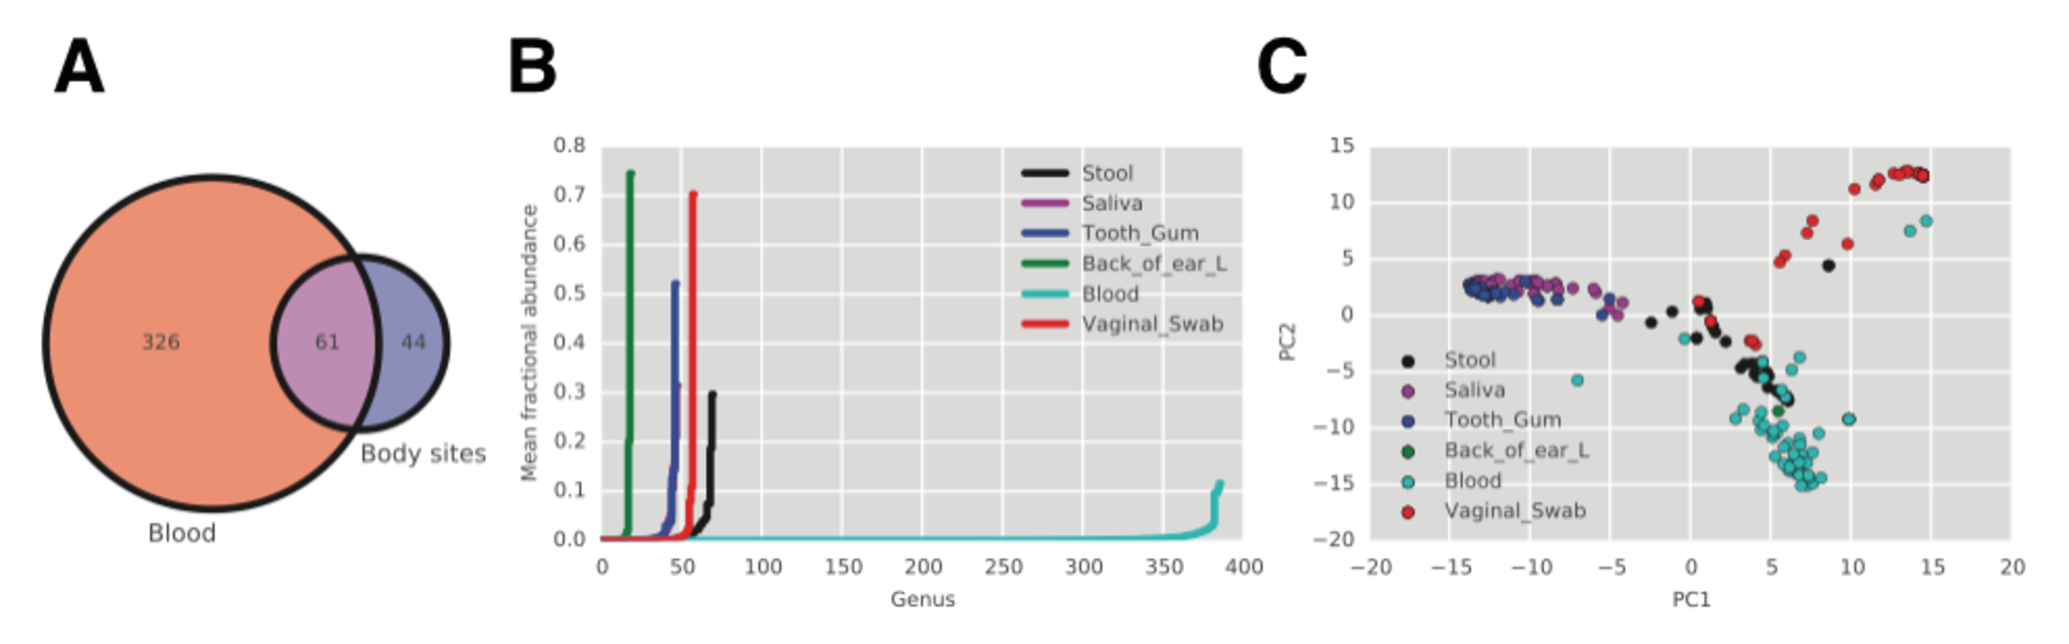
\includegraphics[width=150mm,scale=0.5]{Figures/Fig12}
\caption{Composition of the blood microbiome}
\label{fig:Fig12}
\end{figure*}

We next investigated whether blood samples microorganisms from each site. We reasoned that body-site specific micro-organisms provide a reasonable indicator for this. We compute specificity simply by discretizing the genus found in each body site and comparing there to genus found in all other sites (Figure ~\ref{fig:Fig13}). To aid this analysis, we used our sampled body site data as well as the metagenomic community profiles made available by the Human Microbiome Project \cite{Consortium:2012bb}, which contains 35 billion reads taken from 690 samples from 300 US subjects, across 15 body site. In both cases, we computed a list of body-site specific genus, which are only detected in single body sites for all sampled collected. We then asked whether these genus were detected in blood: we detected $57$\% and $45$\% of the site-specific genus in blood using site-specific genus determined via HMP and this study, respectively. We investigated the body site abundance of specific genus found in blood relative to those absent from blood. We found no significant difference between the abundance in either partition, which argues against the possibility that all site-specific genus were found in blood, but under-sampling frustrated their detection.

\begin{figure*}
\center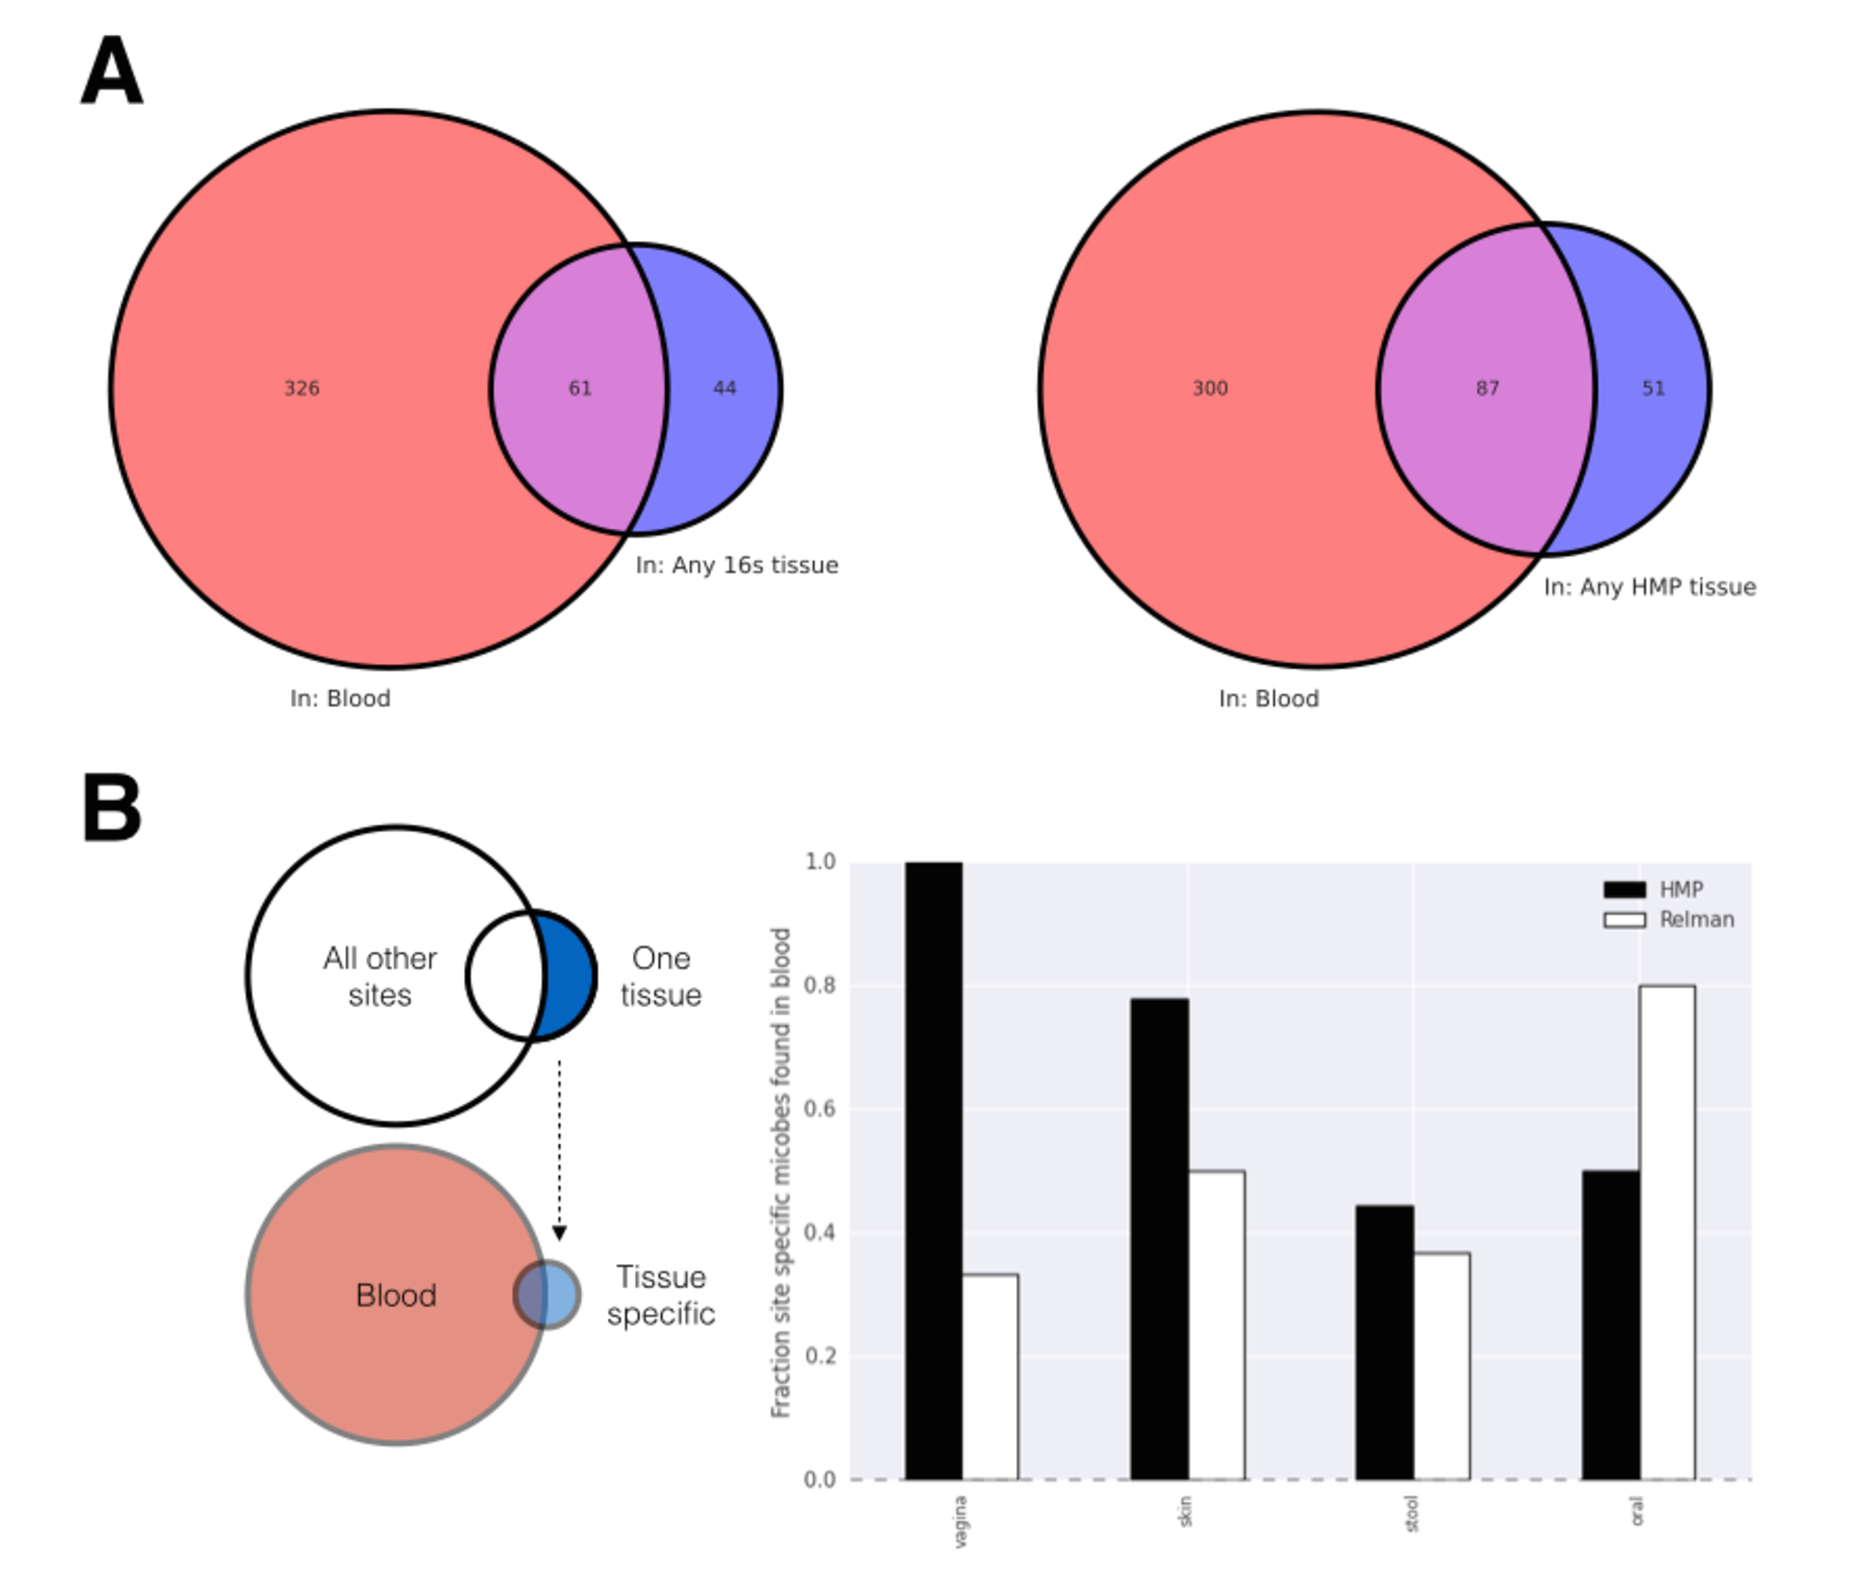
\includegraphics[width=150mm,scale=0.5]{Figures/Fig13}
\caption{Detection of body site specific bacteria in blood}
\label{fig:Fig13}
\end{figure*}

From this analysis, we obtained an assignment of body site specific for each genus detected in our data. In turn, any genus could be assigned to a specific body site or mixed, meaning that it was detected in more than one tissue. We partitioned the genus detected in blood using this assignment in order to understand the origin of genus found in blood. These indicate that blood is composed primarily of two type: genus derived from mixed sources, which cannot be traced to any specific tissue, and genus that are specific to blood only (Figure ~\ref{fig:Fig14}).

\begin{figure*}
\center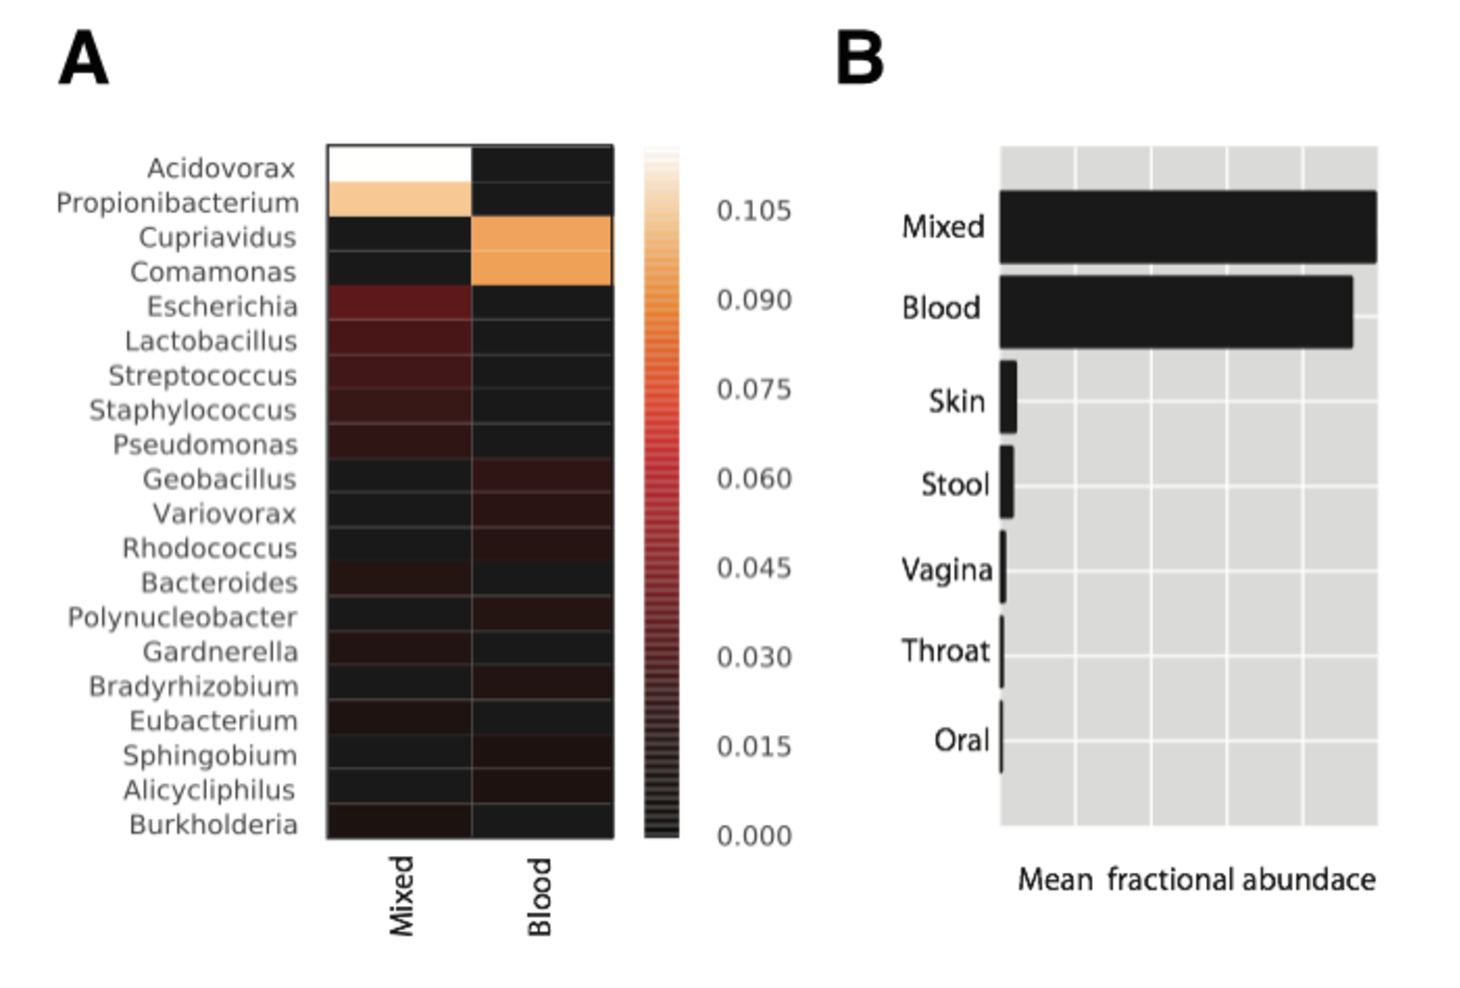
\includegraphics[width=150mm,scale=0.5]{Figures/Fig14}
\caption{}
\label{fig:Fig14}
\end{figure*}

\section{Coupling between blood and body sites}

We then asked if a physical relationship between blood and the body sites can be established based upon the data. Specifically, we examine whether the fractional abundance of genus at each body sites is linked to detection in blood. We discretized the blood data for each sample. For each genus, we then evaluated the fractional abundance of that genus for all matched body site samples. We then compared the distribution of abundances at each body site based upon whether the genus was found in blood, expecting a difference (e.g., an elevation in abundance at a tissue) if there was coupling to blood (e.g., when the genus was found in blood). We found no signifiant evidence of coupling for all genus - body site combinations. 

We further examined whether the composition of blood can be modeled as a function of the sampled sites. We chose a linear model, meaning that each blood sample is modeled as a linear combination of the genus at temporally matched body sites. We used a quadratic programming package to determine for mixing coefficients that minimize the squared error between the model and the blood measurement, subject to intuitive constraints (e.g., the coefficients must be greater than zero). After confirming the model performed correctly on mock data, we applied it to all samples. We found that the model performed poorly, using coefficient of determination ($R^2$) between guess and actually blood data as a measure of performance. We examined residuals to understand the failure, and found - intuitively - that the model fails because many highly abundant genus in blood are not found in the sampled body sites. In order words, the sampled sources are insufficient to describe the composition of blood, as blood apparently sampled from additional sources or serves as an environment that amplifies specific genus non-linearly.

\section{Summary}

The distribution of fractional abundance for genus detected in blood has a different shape than the sampled body sites: blood contains many more genus, but at far lower fractional abundance, with a long tail of genus found at trace abundance. In contrast, sampled body sites are dominated by few genus at high abundance and a relatively short tail of low-abudnance genus. This reflects the fact that some genus are well-adapted to each body site niche. In turn, blood may serve as a common sink into which all tissues contribute dead cells, resulting in a passive environment of mixed DNA fragments that we sampled. We also found that most abundant genus in blood are essentially absent from sampled body sites. This suggests that either that blood can samples from more sources (e.g., internal tissues) or that blood may be a niche for a certain, narrow sub-set of genus. 

Analysis of site-specific genus provides evidence that blood samples each body site, as around half of site specific genus are found in blood when analyzed at both genus and species-level resolution using both our body site data as well as the HMP data. However, we did not find clear evidence of coupling between body sites and blood: there is not apparent difference in genus abundance at any body site based upon whether that genus is detected in blood in a temporally matched sample. This is not surprising: the blood is under-sampled, meaning that few of the present microorgaism-dervied fragments are actually sequenced in our data, and blood is a complex mixture represent many tissue sources. The latter point also frustrated efforts to model blood as a function of the sampled sites: blood data contains genus that were not detected in any of the sampled tissues. 
